\documentclass[apj]{emulateapj}
\usepackage{apjfonts,amsmath,natbib}

\slugcomment{\texttt{draft 2010-12-01 / not ready for distribution}}
\shorttitle{\textsc{data-driven spectral modeling}}
\shortauthors{\textsc{tsalmantza \& hogg}}
\newcommand{\project}[1]{\textsl{#1}}
\newcommand{\sdss}{\project{SDSS}}
\newcommand{\SDSS}{\sdss}

\begin{document}

\title{A data-driven model for spectra:\\
       finding double redshifts in the \SDSS}
\author{P.~Tsalmantza\altaffilmark{1} and David~W.~Hogg\altaffilmark{1,2}}
\email{vivitsal@mpia.de}
\altaffiltext{1}{Max-Planck-Institut f\"ur Astronomie, K\"onigstuhl 17, 69117 Heidelberg, Germany}
\altaffiltext{2}{Center~for~Cosmology~and~Particle~Physics, Department~of~Physics, New York University}

\begin{abstract}
We present a data-driven method---heteroscedastic matrix
factorization---for modeling or performing dimensionality reduction on
observed spectra.  The method uses an iterative
inverse-variance-weighted least-squares minimization procedure to
generate a best set of basis functions.  The method is similar to
principal components analysis, but with the substantial advantage that
it uses measurement uncertainties in a responsible way and accounts
naturally for poorly measured and missing data; it models the variance
in the noise-deconvolved data space.  A regularization can be applied,
in the form of a smoothness prior (inspired by Gaussian processes) or
a non-negative constraint, without making the method prohibitively
slow.  Because the method optimizes a justified scalar (related to the
logarithm of the likelihood), the basis provides a better fit to the
data in a probabilistic sense than any PCA basis.  We test the method
on \SDSS\ spectra, concentrating on spectra known to contain two
redshift components: These are spectra of gravitational lens
candidates and super-massive black-hole binaries (SMBHBs). We apply a
hypothesis test to compare one-redshift and two-redshift models for
these spectra, utilizing the data-driven model trained on a random
subset of all \SDSS\ spectra.  This test confirms 129 of the 131 lens
candidates in our sample and all 4 of the known SMBHB candidates, and
turns up very few false positives.
\end{abstract}

\keywords{keywords}

\section{Introduction}\label{intro}
Modeling data with data-driven models is necessary for many
applications, in part because it is rare that theoretical models are
specific enough, accurate enough, or rich enough to generate all of
the features of a data set.  Common examples in astronomy come in the
study and analysis of spectra.  Redshift determination (CITE),
emission-line measurements (CITE), and decomposition into different
stellar populations (CITE) can all in principle be performed with
spectral models, but rarely are the spectral models accurate enough or
detailed enough to make measurements as precise as contemporary data
permit.  In addition to the quantitative deficiencies of theoretical
models---the fact that they rarely can explain the data at the
precision of the observations---heoretical models contain qualitative
uncertainties---uncertainties about model assumptions and
computational approximations---that inevitably propagate into
theory-driven models.  For these reasons, the highest-performing
redshift determination systems, for example, use data-driven models
that involve principal components analysis (PCA) or similar approaches
(DWH CITE SDSS).

DWH: OUTLIER DETECTION paragraph.

DWH: CLASSIFICATION paragraph.

The standard data-driven models used for spectroscopic astronomical
data are the highest-ranked principal components from a principal
component analysis (PCA) or equivalent. The PCA has one advantage and
a number of drawbacks.  The advantage is that it is entirely
data-driven: The construction of the PCA requires no theoretical or
external knowledge about the spectra being modeled; it is a
dimensionality reduction in the space of the observed spectra.

There are many drawbacks to PCA but the most important is that the PCA
returns the principal directions---the eigenvectors with maximum
eigenvalues---of the variance tensor of the data; this variance tensor
has contributions from intrinsic variation among spectra, and
contributions from observational noise.  That is, a direction in
spectrum space can enter into the top principal components because it
is a direction of great astrophysical variation, or because there is a
lot of noise in the observations along that direction, or both.  PCA
is agnostic about the source of the variance, while astronomers are
not; astronomers want to know about the astrophysical processes that
generate the data prior to the addition of observational noise.

Other drawbacks to PCA include the following: It treats the data as
drawn from a linear subspace of the full spectral space. This
assumption is unlikely to be true in any application.  It also has
trouble separating the spectral variation that comes from amplitude
changes (overall flux or luminosity changes) as distinct from
variations that come from shape changes in the spectra.  Various hacks
have been employed to deal with this, but many of them make the linear
subspace assumption even less valid than it was \textit{a
  priori}. Finally, PCA has no idea about prior information; it is
just as happy creating components with negative amplitudes as positive
amplitudes and the linear subspace therefore contains many quadrants,
in general, that represent spectra with completely unphysical
properties (such as negative emission lines and the like).

In this paper, we introduce a new data-driven
technique---heteroscedastic matrix factorization (HMF)---for modeling
observed spectra that overcomes some---though not all---of the
problems with PCA.  The principal advantage of HMF over PCA is that
the method optimizes not squared error, but rather the justified
probabilistic objective of $\chi^2$.  This leads to the important
difference with PCA that HMF builds a model of the variance in the
data set \emph{not} introduced by observational noise.  That is, it
returns a model of the noise-deconvolved spectral space, which is the
space of interest to the scientific investigator.

As a natural by-product and with no modifications, HMF also deals
responsibly and correctly with missing data.  HMF does not directly
address the linearity and prior problems with PCA.  However, because
the objective function has a direct likelihood interpretation, it
becomes possible to incorporate its work into a Bayesian inference
with proper prior information.  We give some examples of this below.

At the beginning of this introduction, we mentioned outlier
identification.  Some of the most important outliers found in the
\sdss\ data are HOGG

HOGGGGGG

For a given number of components and with a
set of observed spectra as a training set, the method uses a set of
basis functions as an initialization and estimates the coefficients
that provide the best fit to the data. Then, by keeping that set of
coefficients fixed, it estimates a new set of basis functions that
improves the fit to the spectra of the training set. After a small
number of iterations of these two steps the method converges to the
components with the minimum $\chi^2$ value. The method is presented in
detail in sections \ref{method} and \ref{optimization}. Applications
of this technique are presented in section \ref{applications} where we
confirm known double-redshift objects, such as gravitational lenses
and super-massive black-hole binaries (SMBHBs) in the \sdss. This is
achieved by comparing the fitting of the spectra when we use the
estimated components at the redshift provided by the \sdss\ and when
we use an additional set of components at a second redshift. In almost
all the cases tested here we were able to detect a significant
improvement in the quality of the fit when the object was considered
as a superposition of the linear combination of two sets of components
at different redshifts. The paper closes with a brief discussion in
section \ref{discussion}.

\section{Spectral model}\label{method}
Each of the $N$ observed spectra $i$ can be thought of as an ordered list or column vector $\vec{f}_i$ of $M$ flux density (energy per area per time
per wavelength) measurements $f_{ij}$ on a grid of $M$ observer-frame wavelengths $\lambda^{\mathrm{obs}}_j$:
\begin{equation}\label{e1}
\vec{f}_i
\equiv \left[\begin{array}{c} f_{i1} \\
                              f_{i2} \\
                              \cdots \\
                              f_{iM} \end{array}\right]
\equiv \left[\begin{array}{c} f_{\lambda,i}(\lambda^{\mathrm{obs}}_1) \\
                              f_{\lambda,i}(\lambda^{\mathrm{obs}}_2) \\
                                                \cdots \\
                              f_{\lambda,i}(\lambda^{\mathrm{obs}}_M) \end{array}\right]
\quad ,
\end{equation}
Associated with each measurement $f_{ij}$ is an uncertainty variance $\sigma_{ij}$ and we will assume in what follows that these uncertainty variances are well measured and that the uncertainties are essentially Gaussian.  We will assume that off-diagonal terms (covariances) in the uncertainty variance tensor are small, or that the uncertainty variance tensor (covariance matrix) $\textbf{C}_i$ is approximately
\begin{equation}\label{e2}
\textbf{C}_i =
 \left[\begin{array}{cccc} \sigma_{i1}^2 & 0 & & 0 \\
                           0 & \sigma_{i2}^2 & & 0 \\
                           & & \cdots & \\
                           0 & 0 & & \sigma_{iM}^2 \end{array}\right]
\quad .
\end{equation}

We want to model the spectrum of each object with a sum of $K$ linear components:
\begin{equation}\label{e3}
f_{\lambda}(\lambda) = \sum_{k=1}^{K} a_k\,g_k(\lambda)
\quad ,
\end{equation}
where the modeling is done implicitly in the object rest frame, the $a_k$ are coefficients, and the $g_k(\lambda)$ are basis spectra.
Given basis spectra, the best set of coefficients for any observed spectrum---under the assumption of known, Gaussian uncertainties---are found by least-square fitting.  The challenge is to find the best set of basis spectra.

Often in astronomy, this basis is found by principal component analysis (or equivalent) and then selection of the largest-variance
components or largest-eigenvalue eigenvectors.  However, this use of PCA naturally locates the $K$-dimensional linear basis that minimizes the mean-squared error in the space in which all pixels of all spectra are treated equally: They are weighted equally in the analysis, and residuals in them are minimized by the PCA with equal aggression. This is an inappropriate approach in the real situation in which different data points come with very different uncertainty variances, and it is absolutely inapplicable when there are missing data---as there always are in real data sets.

For these reasons, we seek to find the basis set that optimizes a justified scalar objective, one that is consistent with the individual spectral pixel uncertainty variances and with the fact that there are missing data.  When uncertainties are gaussian with known variances, the logarithm of the likelihood is proportional to chi-squared, so we seek to find the basis functions and coefficients that minimize a total chi-squared:
\begin{eqnarray}\label{e4}\displaystyle
\chi^2 & = & X - 2ln\mathcal{L} \nonumber\\
 & = & \sum_{i=1}^N \sum_{j=1}^M
\frac{\left[f_{ij}-\sum_{k=1}^K a_{ik}
                      \,g_{kj}(\lambda_j/[1+z_i])\right]^2}
{\sigma^2_{ij}}
\quad ,
\end{eqnarray}
where $X$ is some constant and we have implicitly assumed that each spectrum $i$ under consideration at this stage is well explained by having all its flux come from a single object at a known redshift $z_i$. The free parameters are the $N\,K$ coefficients $a_{ik}$ and the $K$ functions $g_k(\lambda)$. Roughly speaking, we seek to find the coefficients and basis functions that globally minimize this scalar $\chi^2$.

Precisely speaking, we make two adjustments to this goal. The first is that we can't demand global optimization; this problem is not
convex.  Indeed, there are enormous numbers of local minima, in both the trivial sense that there are exact degeneracies (swap two basis functions and their corresponding coefficients, or re-scale a basis function and the corresponding coefficients, and so on) and in the non-trivial sense that there are qualitatively different solutions. All that our methods (described in detail below) guarantee is that we have, at fixed coefficients $a_{ik}$ the globally optimal basis functions $g_k(\lambda)$ and that we have, at fixed basis functions $g_k(\lambda)$ the globally optimal coefficients $a_{ik}$.

The second adjustment is that we impose a smoothness prior to improve performance at (rest-frame) wavelengths at which we have very few data. In practice, we implement this prior by constructing the basis functions $g_k(\lambda)$ on a grid of $M_g>M$ rest wavelengths $\lambda_{\ell}$ and penalizing quadratically large pixel-to-pixel variations. That is, we optimize not the pure $\chi^2$ above but a modified scalar $\chi_{\epsilon}^2$
\begin{equation}\label{e5}
\chi_{\epsilon}^2 \equiv \chi^2
 + \epsilon\,\sum_{k=1}^K \sum_{\ell=2}^{M_g}
 \left[g_k(\lambda_{\ell})-g_k(\lambda_{\ell-1})\right]^2
\quad ,
\end{equation}
where $\epsilon$ is a scalar that sets the strength of the smoothing. Optimization of this scalar $\chi_{\epsilon}^2$ is equivalent to
optimization of the posterior probability distribution with a Gaussian prior applied to the pixel-to-pixel differences.

\textbf{discussion of Gaussian Processes and this being like a prior}

The basis functions extracted by minimizing equation \ref{e5} are not restricted to be non-negative. This can lead to solutions that lack physical meaning. For this reason the method also provides the possibility of using a non-negative constraint for the components and the coefficients. To proceed with the optimization in this case we start with an all-positive first guess and then iterate these multiplicative updates (Blanton \& Roweis \citealt{blanton}):
\begin{equation}\label{e6}
a_{ik} \gets a_{ik}\left[\sum_{j=1}^{M}\frac{1}{\sigma^2_{ij}}f_{ij}g_{kj}\right]\left[\sum_{n=1}^{K}\sum_{j=1}^{M}\frac{1}{\sigma^2_{ij}}a_{in}g_{nj}g_{kj}\right]^{-1}
\quad ,
\end{equation}
\begin{equation}\label{e7}
g_{kj} \gets g_{kj}\left[\sum_{i=1}^{N}\frac{1}{\sigma^2_{ij}}f_{ij}a_{ik}\right]\left[\sum_{n=1}^{K}\sum_{i=1}^{N}\frac{1}{\sigma^2_{ij}}a_{ik}g_{in}g_{nj}\right]^{-1}
\quad ,
\end{equation}

As is obvious from those equations, the presence of negative fluxes $f_{ij}$ in the observed spectra could lead to negative solutions for the estimated components and coefficients. For this reason, before we apply the method to the observed training set, all the negative fluxes and their corresponding errors are set to zero. In this way the data of those pixels is not taken into account when we use equations \ref{e6} and \ref{e7}.

\section{Optimization}\label{optimization}
As already mentioned, the problem of defining the best basis functions for modeling a set of observed spectra is not convex, and there are multiple minima, including degenerate solutions. We optimize to a local minimum using iterated least squares. In each step, we fix the $g_{kj}$ and find the optimal $a_{ik}$ by weighted least squares, and then hold the $a_{ik}$ fixed and find the optimal $g_{kj}$ by weighted least squares. Each iteration step is guaranteed to reduce the total $\chi^2$ and converges in practice in ten or so iterations. We initialize the fitting with the output of a PCA on the spectra after each spectrum has been projected into a subspace orthogonal to the mean spectrum of the data set; the first guesses for the $g_{k}$ are set to the mean spectrum and the first $K-1$ principal components.

We find that performance is not worse if we use different initializations. In section \ref{training} we demonstrate this by applying the method to a set of SDSS spectra when we use PCA or K-means results (\textbf{ref}), a randomly chosen set of spectra, or functions like sin and cosin for the initialization. For the case that non-negative constraints are applied to the estimated components and coefficients (see equations \ref{e6} and \ref{e7}), we are forced to use an initialization with positive values. Even though we could use any set of positive basis functions, the best initialization seems to be the results of the K-means algorithm. That is expected since the components extracted by K-means, that correspond to the centers of the groups into which the algorithm divides the training spectra, include more physical information than other non-negative initializations. We expect that the K-means results will include only positive values because if the number of groups is not very large (this might result in groups with very few spectra as members), the mean spectrum in each group very rarely includes negative values of flux caused by errors.

Importantly in the training, the wavelengths $\lambda_j$ are rest-frame wavelengths, and because different training-set spectra were taken at different redshifts, not all spectra have coverage at all rest-frame wavelengths. Additionally there are also gaps from bad sky subtraction, cosmic rays, and other data issues.  Missing data in spectrum $i$ at wavelength $j$ is handled naturally by setting
$1/\sigma^2_{ij}$ to a very small value; when a data point has vanishing inverse variance, it does not contribute to $\chi^2$ or the fitting. In general, weighted least squares---because it uses the error variances correctly---is unperturbed by missing data.

For any $K$-dimensional linear subspace, there are many choices for the components $g_k$: The components can be reordered, multiplied
by scalars, or replaced with linear combinations of themselves.  We don't try to break all of these degeneracies, but we do enforce the constraint that the $\vec{g}_k\cdot\vec{g}_k=1$, where the inner product is taken with the trivial (identity) metric in the spectrum space. Additionally we rotate the system of the basis functions and reorder the components according to the variance they include:
\begin{equation}\label{e8}
\sum_{i=1}^{N}a_{ik}>\sum_{i=1}^{N}a_{i(k+1)}
\end{equation}

It should be mentioned that the last step (i.e. equation \ref{e8}) is not used in the case that non-negative constrains are applied.

To speed up the process of extracting the basis $g_{k}$ that minimizes the total $\chi^2$ for a given set of coefficients $a_{k}$ we have implimented two different methods: i) a block-diagonal (or nearly so) least-square fitting and ii) an iterated gradient descent. In the first case we approximate equation \ref{e5} with:
\begin{equation}\label{e9}
\begin{array}{rcl}
\chi^2_{J} & \equiv & \sum_{i=1}^{N}\frac{(f_{iJ}-\sum_{k=1}^{K}a_{ik}g_{kJ})^2}{\sigma^2_{iJ}}+\epsilon\sum_{k=1}^{K}(g_{kJ}-g_{k(J+1)})^2+ \\
&&\\
 & & +\epsilon\sum_{k=1}^{K}(g_{k(J-1)}-g_{kJ})^2
\quad 
\end{array}
\end{equation}

Using equation \ref{e9} we can minimize the $\chi^2$ value for each wavelength J and define the new set of basis functions. Since the estimation of the component values at the Jth pixel requires their values at the (J+1) and (J-1) pixels, we make use of the values that the components had in those pixels at the previous iteration.

When using conjugate gradient descent we update the coefficients based on the equations (Shewchuk \citealt{shewchuk}):
\begin{equation}\label{e10}
a_{ik} \gets a_{ik}+\alpha r_{ik}
\quad ,
\end{equation}

where:
\begin{equation}\label{e11}
r_{ik}=\frac{f_{ij}-\sum_{k=1}^{K}a_{ik}g_{kj}}{\sigma^2_{ij}}g_{jk}
\quad ,
\end{equation}
\begin{equation}\label{e12}
\alpha=\frac{\sum_{i=1}^{N}\sum_{k=1}^{K}r^2_{ik}}{\sum_{i=1}^{N}\sum_{k=1}^{K}r_{ik}R_{ik}}
\quad ,
\end{equation}
\begin{equation}\label{e13}
R_{ik}=\frac{r_{ik}g_{kj}}{\sigma^2_{ij}}g_{jk}
\quad ,
\end{equation}

and the basis functions:
\begin{equation}\label{e14}
g_{kj} \gets a_{kj}+\beta p_{ik}
\quad ,
\end{equation}
\begin{equation}\label{e15}
q_{kj}=a_{ki}\frac{f_{ij}-\sum_{k=1}^{K}a_{ik}g_{kj}}{\sigma^2_{ij}}+\epsilon(g_{k(j+1)}-g_{kj})+\epsilon(g_{k(j-1)}-g_{kj})
\quad ,
\end{equation}
\begin{equation}\label{e16}
\beta=\frac{\sum_{k=1}^{K}\sum_{j=1}^{M}q^2_{ik}}{\sum_{k=1}^{K}\sum_{j=1}^{M}q_{kj}Q_{kj}}
\quad ,
\end{equation}
\begin{equation}\label{e17}
Q_{kj}=a_{ki}\frac{a_{ik}q_{kj}}{\sigma^2_{ij}}-\epsilon(q_{k(j+1)}-q_{kj})-\epsilon(q_{k(j-1)}-q_{kj})
\quad ,
\end{equation}

By comparing the two methods, through tests performed with SDSS spectra, we see that even though the use of the gradient descent is much faster at each iteration than the block diagonal case, it requires many more iterations in order to converge to the same results. This makes the first option faster and for that reason, it is the one used for the results presented below.

In the case with non-negative constrains the solution of equations \ref{e6} and \ref{e7} is very fast, allowing us to perform a large number of iterations ($\approx 10^3$) until they converge. To decrease the number of iterations, we iterate equation \ref{e6} many times ($\approx 10^2$) during the initialization while keeping the initial basis fixed, in order to optimize the set of initial coefficients.

\section{Applications}\label{applications}
To assess the power of the technique, we are going to confirm known double-redshift objects in the SDSS spectroscopic sample. More specifically, by using the method presented above, we define a small number of components that is sufficient for modeling the SDSS spectra. Using these components we fit each observed spectrum at the redshift provided by SDSS. Then we repeat the fitting, but this time using one set of components at the SDSS redshift and one set of components at values of redshift that lie on a nominal grid. If a second object is present we expect the fit to be improved when we use two sets of components, one at the redshift of SDSS and one at that of the second object. In the examples that follow we will demonstrate this using the SLACS sample of gravitational lenses (Bolton et al. \citealt{bolton}) and the four known candidates of Supermassive Black Hole Binaries (SMBHBs) (\textbf{ref}).

\subsection{Training}\label{training}
In order to detect the presence of two objects at different redshifts in the SDSS spectra, we need to be able to model the spectra of all types of objects that have been observed by the survey (galaxies, LRGs and QSOs). To do so, we have to train our method separately for each class. For this purpose we selected a small random sample of spectra for each type of object (approximately 5000 for galaxies and LRGs and 10000 for QSOs, the numbers were selected as such in order to make sure that we have at least as many objects as number of pixels, which was needed for some of the tests we performed using PCA). The spectra were taken from the 7th Data Release (DR7) of SDSS (\textbf{ref}). The values of redshift were selected to be in the ranges of  0.01-0.06, 0.20-0.50 and 0.10-1.50 for galaxies, LRGs and QSOs respectively.

For the selection of the LRG sample used in this study we followed the target selection of the LRG sample in SDSS which is based on 2 cuts, defined using magnitudes, colors and surface brightness criteria (Eisenstein et al. \citealt{eisenstein}). Cut I is suitable for selecting LRGs with z$<$0.4 and CUT II for LRGs with z$>$0.4. According to Eisenstein et al. \cite{eisenstein} these criteria are suitable for redshifts in the range of values greater than 0.15 and less than 0.55. The number of galaxies fulfilling these criteria is expected to be about 100,000 by the end of the survey. The primTarget field that is provided in the SpecObjAll table of SDSS is set to GALAXY\_RED if the LRG passes either CUT I or CUTII and to GALAXY\_RED\_II if it passes CUTII but not CUTI. For this study we downloaded the data for the LRGs that had their primTarget equal to either GALAXY\_RED and GALAXY\_RED\_II and only GALAXY\_RED (since if the primTarget is set as GALAXY\_RED\_II it is by default set as GALAXY\_RED as well).

The sample was used to determine the maximum wavelength coverage, i.e. a wavelength area for which at least 10 sources have valid data at the beginning and the end of the spectrum. In this way we are able to fit the part of the spectrum that is produced by the second object for a large range of redshift values. During this procedure, pixels with any of the flags: SP\_MASK\_FULLREJECT, SP\_MASK\_NODATA, SP\_MASK\_BRIGHTSKY, SP\_MASK\_NOSKY or pixels that correspond to zero noise were treated as masked. All the spectra and their noise were moved to the rest-frame by keeping the energy constant in each spectral bin while relabeling the wavelength axis.  The final wavelength coverage for each object is: 3580.964-9109.615 \AA\ for galaxies, 2544.486-7615.528 \AA\ for LRGs and 1522.299-8352.183 \AA\ for QSOs, corresponding to 4056, 4762 and 7394 pixels respectively. Since only 10 spectra include data at the bluest and reddest wavelengths, missing data is present in almost all the spectra of our sample. To deal with this problem we have set the fluxes at those areas equal to the first or the last non-masked pixel of the spectrum and we have set the noise of those pixels to a very high value ($10^{-12} erg/sec/cm^2/$\AA), so that they will not be taken into account by the method. As a last step before the application of the method all spectra were interpolated to the wavelengths selected for each type of source using cubic splines. The selected wavelengths are uniformly distributed in log space as in the case of the original SDSS wavelengths. For the resulting spectra we interpolated linearly the values of the masked pixels.

Using a number of spectra equal to the number of pixels selected for each source, we performed PCA on those data. The training data were first normalized in a way that all spectra were moved to a hyperplane passing from the zero point and perpendicular to the mean spectrum. Additionally the flux in each spectral bin has been divided with the RMS of the noise in that bin for all the non-masked pixels in the training sample. The PCA results were used as an initialization to our method. The method was run for a subset of approximately 1000 spectra of each type for a different number of components and for 16 iterations, which seems to be enough for the method to converge. This can be seen in figure \ref{f1} in which we present the results of the fitting (total $\chi^2$, i.e. the sum of $\chi^2$ values over all wavelengths and all spectra) of the 1000 spectra of our sample with a different number of components. This test was also performed for four different values (1,3,10 and 30) of the smoothing factor $\epsilon$.

\begin{figure}[h]
% \includegraphics[angle=-90,width=0.99\columnwidth]{paper_plots/fig1.ps}
\caption{The total $\chi^2$ value estimated by the fit of the training set of spectra by the components produced by the method vs. the number of components for each type of object (rows) and values of $\epsilon$ (columns).}
\label{f1}
\end{figure}

In figure \ref{f1} we can see that the fitting of the spectra improves a lot even after the first iteration, indicating that using this method and a given number of components we can achieve a better modeling of the spectra than with the PCA. In figure \ref{f2} that follows we present our new set of components plotted over the initial PCA components. We should point out that a straight comparison between the components extracted by the two methods is not meaningful since they correspond to different subspaces of the observed data and that the comparison between the methods can be achieved only by using the results of the fitting to a set of spectra.

\begin{figure}[h]
\begin{center}
%\includegraphics[angle=-90,width=0.99\columnwidth]{paper_plots/fig2.ps}
%\includegraphics[angle=-90,width=0.99\columnwidth]{paper_plots/fig3.ps}
%\includegraphics[angle=-90,width=0.99\columnwidth]{paper_plots/fig4.ps}
\caption{The first 7 components for each type of object (galaxies, LRGS and QSOs) as estimated by the PCA (grey lines) and the method presented here (black lines).}
\label{f2}
\end{center}
\end{figure}

In figure \ref{f1} we also present how the components and the total $\chi^2$ value change with the value of the smoothing factor $\epsilon$. As was expected, by increasing the value of the $\epsilon$ parameter, and therefore the smoothness of the resulting components, we put more constraints on them, leading to worse fits of the data.

In the results presented above (figure \ref{f1}) we have used the same set of data to train as well as to test the method. As a first step towards cross-validation we used a new random set of 1000 spectra as a testing set. The results of the fitting of this set, at each iteration, with the components we extracted with the method and the same training set of spectra as before, are presented in figure \ref{f3}. In these plots with different types of line we present the results for different values of $\epsilon$. As we can see in the new test set the best fit is achieved by different values of $\epsilon$ and not for the smallest one as before.

\begin{figure}[h]
%\includegraphics[angle=-90,width=0.99\columnwidth]{paper_plots/fig5.ps}
\caption{The total $\chi^2$ value estimated by the fit of the test set of spectra by the components produced by the method vs. the number of components for each type of object (rows: galaxies, LRGs and QSOs respectively). The different types of lines represent the different values of $\epsilon$ used in each case.}
\label{f3}
\end{figure}

In order to check how much the method depends on the initialization we repeated our tests using different sets of components as our initial basis. In figure \ref{f4} we present the results of the fitting for the same test set as before when we used a random set of spectra, the output of the K-means algorithm and a set of sin and cosin functions to initialize the method. More specifically in the case that a set of random spectra was used, we selected the ones that include information at the reddest or the bluest part of the spectrum. In the case of the K-means initialization we used the algorithm kmeans(stats) implemented in R with a number of centers equal to the number of components needed. The algorithm uses a random set of points as its initialization and therefore the results are slightly different in every run.

\begin{figure}[h]
%\includegraphics[angle=-90,width=0.99\columnwidth]{paper_plots/fig6.ps}
\caption{The total $\chi^2$ value estimated by the fit of the test set of galaxy spectra by the components produced by the method vs. the number of components. The different types of lines represent the different initializations used (PCA, K-means, random spectra and sin and cosin functions).}
\label{f4}
\end{figure}

By comparing these results we see that they are becoming worse as we change the initialization from the PCA output, to the random spectra, to the K-means results and to the sin and cosin functions. This result is expected since the PCA results are chosen in a way to increase the percentage of the total variance they include. The most probable reason why the random spectra seem to be a better initialization than the K-means output is that we have chosen spectra that include information at the ends of the wavelength coverage, something that is probably not true in the K-means initialization where the centers are defined mainly by spectra with constant values in these areas. The sin and cosin functions lead to the worst results as expected since they include the least information compared to all the other initializations used here.

As a last test of the method we checked how a non-negative constraint affects the results. Since negative values in the spectra are caused by observational errors, modeling the spectra of astronomical sources with components that include negative values has no physical meaning. This problem can be solved be applying a non-negative constraint to our basis. The way that this is achieved is by initializing with a non-negative set of components and coefficients and iterating according to equations \ref{e6} and \ref{e7}. One of the best ways to initialize this method with a set of non-negative components that include physical information is to use once again the K-means algorithm. The results of the fitting of the test set of spectra with the components extracted in this way after 2048 iterations are presented in figure \ref{f4}, while in figure \ref{f5} we present the resulting components for each type of object for K=7.

\begin{figure}[h]
\begin{center}
%\includegraphics[angle=-90,width=0.99\columnwidth]{paper_plots/fig7.ps}
%\includegraphics[angle=-90,width=0.99\columnwidth]{paper_plots/fig8.ps}
%\includegraphics[angle=-90,width=0.99\columnwidth]{paper_plots/fig9.ps}
\caption{The first 7 components for each type of object (galaxies, LRGs and QSOs) as estimated by the PCA (grey lines) and the method presented here (black lines) when non-negative constraints were applied.}
\label{f5}
\end{center}
\end{figure}

By comparing those results with the ones obtained without the non-negative constraint we see that the fitting is now worse. This was of course expected since this is a very strict constraint. On the other hand even if the components now seem to have a better physical meaning, i.e. they look more like spectra of particular types of objects, in many cases there seems to be a problem at the edges of the spectra where they tend to start from exactly zero values (e.g. the components for LRG objects). At this point we should mention that when applying the method for the non-negative case we have not used an additional smoothing constraint.

Based on the results presented here and an additional test to select the optimum number of components by checking how many are needed in order to detect the second redshifts in the SLACS and SMBHB candidate samples, we have decided to fit the SDSS spectra using the 14, 7 and 14 components that were produced by our method for galaxy, LRG and QSO sources after 16 iterations and using $\epsilon$=3, 30 and 10 respectively. It is interesting that fewer components are needed in order to fit well the LRG SDSS spectra than the galaxy and QSO ones. This is expected, since the LRG spectra have less variation. A more detailed description of the fitting and its results is presented below.

\subsection{Hypothesis test}\label{hypothesis}
In order to detect the presence of a second redshift in the SDSS spectra for each spectrum $i$, we generate $Z+1$ mutually exclusive hypotheses: The null hypothesis $S_i$ that spectrum $i$ only has significant flux coming from a single redshift $z_i$ determined by the \facility{SDSS} pipeline, and $Z$ hypotheses $D_{im}$ that spectrum $i$ has significant flux coming from two redshifts, $z_m$ and another redshift $z_m>z_i+\epsilon$.  In the context of this very restricted universe of hypotheses, the odds ratio $\Omega_i$ for the null hypothesis is 
\begin{equation}\label{eq:odds}
\Omega_i = \frac{\sum_{m=1}^Z p(D_{im}|\vec{f}_i,I)}{p(S_i|\vec{f}_i,I)}
 = \sum_{m=1}^Z \left[\frac{p(\vec{f}_i|D_{im},I)}{p(\vec{f}_i|S_i,I)}
 \,\frac{p(D_{im}|I)}{p(S_i|I)}\right] = \sum_{m=1}^Z\Omega_{im}\quad,
\end{equation}
where the spectral flux data are represented by the vector $\vec{f}_i$, the symbol $I$ represents all of the prior information in the problem, including but not limited to the hypothesis specification, the wavelengths and uncertainties associated with the spectral flux data, and any other knowledge that the investigator might have about the hypotheses prior to any data analysis. We have implicitly defined an individual-hypothesis odds ratio
\begin{equation}
\Omega_{im} = \frac{p(\vec{f}_i|D_{im},I)}{p(\vec{f}_i|S_i,I)}
  \,\frac{p(D_{im}|I)}{p(S_i|I)}\quad.
\end{equation}
Because an individual spectrum is unlikely a priori to show two redshifts, the prior probabilities will have the asymmetry
\begin{equation}
\sum_{m=1}^Z p(D_{im}|I) \ll p(S_i|I) \quad,
\end{equation}
and it remains for us to decide how to set the relative prior probabilities among the $Z$ hypotheses $D_{im}$.

We have split the sum in the odds $\Omega_i$ into a sum of individual odds ratios $\Omega_{im}$ because, as we will see, we need to estimate the ratio for each $m$ individually; we can't just evaluate the total numerator and denominator of $\Omega_i$ independently.  The reason for this is the all-important spectral coverage.  Each setting of the pair $(z_i,z_m)$ limits differently the spectral range over which the eigenspectra are both well determined. Imagine that one of the hypotheses $D_{im}$ is only testable in some particular spectral range $[\lambda_{\min},\lambda_{\max}]$.  The data in this spectral range can be used to estimate the single-hypothesis odds ratio $\Omega_{im}$ of hypothesis $D_{im}$ to the null hypothesis $S_i$. Clearly hypotheses $D_{im}$ that are testable with larger spectral ranges will be better tested, but the fact that different hypotheses are subject to tests of different strengths merely weakens---does not invalidate---the total hypothesis test.

The SDSS spectra have near-Gaussian uncertainties. Therefore, for each hypothesis $D_{im}$ we can perform least-square fitting ($\chi^2$ minimization) on the subset of $N_{im}$ pixels in the flux vector $\vec{f}_i$ that overlap the eigenspectra spectral ranges for both redshifts $z_i$ and $z_m$.  If we perform the least-square fit with $n$ eigenspectra at each redshift, then the odds ratio can be approximated by a modified difference in $\chi^2$:
\begin{equation}
\ln\Omega_{im}= \frac{1}{2}\,\left[\chi^2_i-\chi^2_{im}-n\right]
 +\ln\frac{p(D_{im}|I)}{p(S_i|I)} \quad,
\end{equation}
where we have taken the natural logarithm to simplify things, $\chi^2_i$ is the minimum $\chi^2$ under hypothesis $S_i$, $\chi^2_{im}$ is the minimum $\chi^2$ under hypothesis $D_{ij}$, the adjustment of $-n$ accounts for the fact that the $S_i$ fit has $n$ fewer parameters than the $D_{im}$ fit, and the last term is the prior ratio. Importantly, in this odds-ratio expression, the $\chi^2$ fits
for hypotheses $S_i$ and $D_{im}$ must have been performed over the same $N_{im}$ pixels in both cases. Even then, the expression is
something of an approximation, because it effectively assumes that the data are affected by perfectly known, perfectly Gaussian noise and
that one of the two hypotheses is capable of providing a good fit to the data.

In the section that follows we apply this hypothesis test to the spectra of known double redshift sources in SDSS using as basis functions for the fitting, the components extracted in section \ref{training} for each type of object.

\subsection{Testing}\label{testing}

\subsubsection{The SLACS survey}\label{slacs}
The SLACS survey (Bolton et al. \citealt{bolton}) includes 131 strong galaxy-galaxy gravitational lens candidates, selected by the presence of higher redshift emission lines and lower redshift continuum. Using the components extracted by the method presented here (section \ref{training}) for galaxy and LRG SDSS spectra we try to apply the hypothesis test described above and reproduce the results of the SLACS survey for the second redshift.

As a first step we applied the test using the 14 galaxy components of section \ref{training} for both the foreground and the background object. Each spectrum of the SLACS survey was fitted once with the components at the SDSS redshift and the $\chi^2$ value of the fit was calculated. Then the spectrum was fitted again with one set of components at the SDSS redshift and one set of components at a redshift scanning a regular grid of values. The difference between the two $\chi^2$ values (with one and two sets of components) was used to search for peaks in the second redshift. For the case that both sets of components used correspond to galaxy spectra, we detected peaks for 120 SLACS spectra at the same redshifts as in the SLACS survey (figure \ref{f6}). An additional criterium that we used was that the peaks (if present) should correspond to fits that did not produce negative OIII lines if they were included in the spectral range of the fit.

For the remaining 11 cases we applied the same proceedure but this time using the LRG components to fit the foreground object and the galaxy components to fit the background one. The results show that using our method we are extracting the same results as the SLACS survey for 6 of those spectra (figure \ref{f7}).

For the 5 remaining spectra we detect a different second redshift than the one provided by Bolton et al. \cite{bolton}. For those objects we applied once again our method but this time assuming the presence of three objects instead of two. More specifically we fit the spectrum using a set of components (LRG or galaxy) at the SDSS redshift, a set of components (galaxy) at the second redshift to which was given the highest probability according to our method, and a set of components (galaxy) at a redshift scanning a regular grid of values. This time we managed to predict the SLACS second redshift for 3 additional objects (figure \ref{f8}).

For only 2 out of the 131 spectra tested here were we not able to detect their second redshift. The results for these spectra as well as the fitting at the second redshift given by SLACS are shown in figure \ref{f9}. From this figure we see that this is a weak detection with no obvious signature of an additional object at the second redshift.

The results of the method presented here when applied to the SLACS survey are very promising. Our goal is to apply this method to the whole SDSS spectroscopic sample in order to detect new gravitational lens candidates.

\subsubsection{The known sample of SMBHB candidates}\label{smbhb}
Another type of object that can be detected by the presence of two redshifts in its spectrum is the SMBHBs. In the case of SMBHBs we expect the presence of two sets of emission lines (one broad and one narrow) with a small separation between them, caused by the rotation of the less massive black hole around the more massive one that is located at the center of the system. Only four spectra in SDSS have been selected to be SMBHB candidates (\textbf{ref}). By applying our method to those spectra we followed the same procedure as in the case of gravitational lenses in order to test if we can detect the second redshift. However, since in this case the separation between the two sets of lines is expected to be very small, we limited our search to redshifts with a difference from the one provided by SDSS less than 0.1. The second redshift can be either smaller or larger than the SDSS one, depending on the phase of the less massive black hole.

Once again the spectra were fitted using a set of components that were extracted in section \ref{training} for QSOs at the SDSS redshift and one set of the same components at a redshift scanning a narrow grid of regular values. The results for the four candidates are presented in figure \ref{f6a} where we can see that we are able to detect all of the four second redshifts that are given in the literature.

In the future we plan to apply this method to the whole sample of QSO spectra in SDSS in order to detect more candidates of this type of object.

\begin{figure}[h]
%\includegraphics[angle=-90,width=0.49\columnwidth]{paper_plots/1qq.ps}
%\includegraphics[angle=-90,width=0.49\columnwidth]{paper_plots/2qq.ps}
%\includegraphics[angle=-90,width=0.49\columnwidth]{paper_plots/3qq.ps}
%\includegraphics[angle=-90,width=0.49\columnwidth]{paper_plots/4qq.ps}
\caption{The four known SMBHB candidates. \textbf{Top panel:} The $\chi^2$ difference between the fitting of the spectrum with 1 and 2 sets of components. The green and blue lines represent the SDSS redshift and the one with the largest $\chi^2$ difference. \textbf{2nd panel:} The fitting of the spectrum (black) with both sets of components (red). \textbf{3rd panel:} The part of the spectrum (black) fitted by the one set of components at the redshift with the highest $\chi^2$ difference (red). \textbf{Bottom panel:} The part of the spectrum (black) fitted by the one set of components at the SDSS redshift (red).}
\label{f6a}
\end{figure}

\section{Discussion}\label{discussion}
We have developed a new technique based on iterative least-square minimization to model observed spectra. The method is based on estimating the minimum number of components whose linear combination can reproduce well the whole training set of the observations. In order to define the optimal number (K) of components we train the method for different values of K and then we use the produced components to fit a test set of observed spectra. By checking the changes in the total $\chi^2$ value of the fit with the number of components we can define the minimum number that should be used. An additional test for objectively choosing K for specific problems is to use the components extracted by the method for different values of K in order to reproduce accurately the results of known examples.

For the training part of the method we use a subset of the observed spectra to which we want to apply the results. A way to improve the results would be to use the whole set of spectra, except the one under testing, in order to train the method. However, this is a very time consuming procedure, almost impossible in the case of large surveys like SDSS, and for that reason we choose to use a subsample of the data for training purposes.

Another way to improve the results, could be to add prior information on the amplitudes. Based on the coefficients extracted by the fitting of the training spectra by the components, we can draw conclusions about the amplitudes that will occur when the fitting is done for the testing spectra. This way outliers could be detected and unrealistic solutions could be excluded. However, this is also a subject that depends on the size of the training sample and the fraction of the observed variance that it covers. If the training sample doesn't fulfill these criteria then it is possible to produce worse results instead of improving the performance.

In comparison to PCA the method presented here has the advantage of taking into account the errors in the observations. This will lead to components that include more physical information since they are not affected by the variance in the spectra caused by problems or artifacts during the observations. Additionally, since this method is based on the minimization of the total $\chi^2$ value instead of maximization of the variance included in the top components, it produces basis functions that fit the real data much better than the PCA results, for the same number of components, even from the first iteration. Finally, in contrast to PCA the method is also able to handle missing data. This is a big advantage since it allows us to increase the amount of information in the training set by including more objects that we wouldn't be able to use with PCA. An example of this is that we managed to achieve maximum wavelength coverage in the final components even though the training set included objects in a large range of redshifts. However, PCA has an advantage compared to our method which is its time efficiency. Even though techniques like block-diagonal and gradient descent seem to improve the speed of the $\chi^2$ minimization performed, the iterations needed make the method still much slower than PCA. This is an issue that we seek to improve in the future.

Another problem of the method is the existence of many local minima in the resulting basis space. However, this can be solved by using many different initializations and using the results that produce the best fit to the test data. We should point out once again that comparison between the resulting components extracted from different initializations (or different methods) shouldn't be done by straight comparison between the components themselves but by camparing the quality of the fit to a test set of data.

An additional advantage of this method compared to the PCA is that it also provides an option for non-negative constrains in the resulting components and coefficients, based on the work of Blanton \& Roweis \cite{blanton}. This option can produce results that do not include unphysical features (e.g. negative emission lines). We should keep in mind though that since this is a very hard constraint, it has a big impact in the results by producing a poorer fit to the observed spectra.

The results of the method were applied to the problem of confirming double redshift objects in SDSS. From the 131 galaxy-galaxy gravitational lenses in the SLACS survey we were able to automatically detect 129, using the components extracted by the method when trained with galaxy and LRG SDSS spectra, to fit the candidates. The confirmation was made by fitting the spectra once with a set of components at the SDSS redshift and once with an additional set of components at a redshift scanning a regular grid of values. The maximum improvement of the fitting when two sets of components at different redshifts were used instead of one set at the SDSS redshift, occurred at the redshift predicted by SLACS for the second object. Similar were the results for the case of the four known SMBHBs candidates where we were able to reproduce all of them. In the future we will perform an automatic search for objects of these types in all the SDSS spectroscopic data. For the case of gravitational lens candidates we are also planning to expand the search for cases that the secondary object is at lower redshift than the primary and that it could also be another type of source (e.g. QSO). Another application of this method could be for the determination of more accurate redshifts for single objects. This application will be very interesting for the case of QSOs at high redshifts and for defining template spectra for redshift estimation of objects that are going to observed by future surveys. This is is another subject that we seek to work on in the near future.

\section{Acknowledgments}
\textbf{The authors would like to thank...}

Funding for the Sloan Digital Sky Survey (SDSS) has been provided by the Alfred P. Sloan Foundation, the Participating Institutions, the National Aeronautics and Space Administration, the National Science Foundation, the U.S. Department of Energy, the Japanese Monbukagakusho, and the Max Planck Society. The SDSS Web site is http://www.sdss.org/. The SDSS is managed by the Astrophysical Research Consortium (ARC) for the Participating Institutions. The Participating Institutions are The University of Chicago, Fermilab, the Institute for Advanced Study, the Japan Participation Group, The Johns Hopkins University, the Korean Scientist Group, Los Alamos National Laboratory, the Max-Planck-Institute for Astronomy (MPIA), the Max-Planck-Institute for Astrophysics (MPA), New Mexico State University, University of Pittsburgh, University of Portsmouth, Princeton University, the United States Naval Observatory, and the University of Washington.

\appendix

\section{Appendix material}\label{appendix}

\begin{figure}[h]
%\includegraphics[angle=-90,width=0.32\columnwidth]{paper_plots/1gg.ps}
%\includegraphics[angle=-90,width=0.32\columnwidth]{paper_plots/2gg.ps}
%\includegraphics[angle=-90,width=0.32\columnwidth]{paper_plots/3gg.ps}
\caption{As figure \ref{f6a} for the case of SLACS candidates that were fitted with two sets of galaxy components.}
\label{f6}
\end{figure}


\begin{figure}[h]
%\includegraphics[angle=-90,width=0.32\columnwidth]{paper_plots/103lg.ps}
%\includegraphics[angle=-90,width=0.32\columnwidth]{paper_plots/18lg.ps}
%\includegraphics[angle=-90,width=0.32\columnwidth]{paper_plots/55lg.ps}
\caption{As figure \ref{f6a} for the case of SLACS candidates that were fitted with one set of LRG components and one set of galaxy components.}
\label{f7}
\end{figure}

\begin{figure}[h]
%\includegraphics[angle=-90,width=0.32\columnwidth]{paper_plots/12ggg.ps}
%\includegraphics[angle=-90,width=0.32\columnwidth]{paper_plots/59lgg.ps}
%\includegraphics[angle=-90,width=0.32\columnwidth]{paper_plots/68lgg.ps}
\caption{As figure \ref{f6a} for the case of SLACS candidates that were fitted with three sets of components (galaxies and LRGs). The bottom pannel shows the fitting of the residuals by two sets of components.}
\label{f8}
\end{figure}

\begin{figure}[h]
\begin{center}
%\includegraphics[angle=-90,width=0.34\columnwidth]{paper_plots/36gg.ps}
%\includegraphics[angle=-90,width=0.34\columnwidth]{paper_plots/36ggSLACS.ps}
%\includegraphics[angle=-90,width=0.34\columnwidth]{paper_plots/66gg.ps}
%\includegraphics[angle=-90,width=0.34\columnwidth]{paper_plots/66ggSLACS.ps}
\caption{The 2 SLACS candidates that couldn't be confirmed by the method presented here. The left plots show the results of the fitting with the second set of components at the second redshift estimated with the method, while the right at the SLACS second redshift.}
\label{f9}
\end{center}
\end{figure}

\begin{thebibliography}{}
\bibitem[2007]{blanton}
Blanton M. R. \& Roweis S. 2007, AJ, 133, 734

\bibitem[2007]{bolton}
Bolton A. S., Burles S., Koopmans L. V. E., True T., Gavazzi R., Moustakas L. A., Wayth R., Schlegel D. J. 2008, ApJ, 682, 964

\bibitem[2001]{eisenstein}
Eisenstein D. J., Annis J., Gunn J. E., Szalay A. S., Connolly A. J., Nichol R. C., Bahcall N. A., Bernardi M., Burles S., Castander F. J. el al. 2001, AJ, 122, 2267

\bibitem[1994]{shewchuk}
Shewchuk J. R. 1994, http://www.cs.cmu.edu/\~quake-papers/painless-conjugate-gradient.pdf
\end{thebibliography}{}

\end{document}

%%
%% End of file `sample.tex'.
